\documentclass[xcolor=dvipsnames,notes]{beamer}
\usecolortheme[named=Brown]{structure}
\usetheme{default}
\setbeamertemplate{navigation symbols}{} 
\usepackage{tikz}
\usetikzlibrary{arrows,decorations.pathmorphing,backgrounds,positioning,fit}
\usetikzlibrary{datavisualization.formats.functions}
\usetikzlibrary{shapes}
\include{macro}
\usepackage{epsfig}
\usepackage{natbib}
\usepackage{graphicx}
\usepackage{multimedia}
\usepackage{verbatim}
\include{acmmacro}
\begin{document}
%\setbeamercolor{titlelike}{fg=gray,bg=white}
%\setbeamercolor{itemize item}{fg=gray,bg=white}
%\setbeamercolor{enumerate item}{fg=gray,bg=white}
%\setbeamercolor{block title}{fg=black,bg=white}
%==============================================
\title{TPG4190 Seismic data acquisition and processing \\
               Imaging}
\author{B. Arntsen}
\institute[NTNU]{
  NTNU\\
  Department of Geoscience and petroleum \\
  \texttt{borge.arntsen@ntnu.no}
}
\date{Trondheim fall 2020}
\begin{frame}
 \titlepage
\end{frame}
%
%==============================================
\begin{frame}{Overview}
%==============================================
\begin{itemize}
  \item Imaging condition
  \item Simplification
  \item Comparison with classical imaging condition
  \end{itemize}
\end{frame}
%---------------------------------
\begin{frame}{Imaging condition}
%---------------------------------
For the forward modeling we have in the time domain
(Equation (13) in lecture 10).
\begin{eqnarray}
   p(\xx,\xx_s,t) = \int dV(\xx') g(\xx,\xx',t)*s(\xx',t) \nonumber\\
               +\int dS(\xx')\, \left[g(\xx,\xx',t)*\nabla p(\xx',\xx_s)-
              p(\xx',\xx_s,t)*\nabla g(\xx,\xx')\right]\cdot \nn(\xx') \nonumber
\end{eqnarray}
However, for modelling we can neglect the surface integral
\begin{eqnarray}
   p(\xx,\xx_s,t) = \int dV(\xx') g(\xx,\xx',t)*s(\xx',t).
&&                   \label{eq:10000}
\end{eqnarray}
\end{frame}
%---------------------------------
\begin{frame}{Imaging condition}
%---------------------------------
For the time reversed focusing we have
(Equation (19) in lecture 10), but with reinsertion of volume integral
for the $s'(\xx,t)$ source
\begin{eqnarray}
 p(\xx,\xx_s,-t)*h(t)=\int dV\, p(\xx,\xx_s,t)*s'(\xx_s,-t) \nonumber\\
+\int dS(\xx')\, \left[p(\xx',\xx_s,-t)*\nabla p(\xx,\xx',t)\right.\nonumber\\
   -\left. p(\xx,\xx',t)*\nabla p(\xx',\xx_s,-t)\right]\cdot \nn(\xx')
&&                   \label{eq:10100}
\end{eqnarray}
Assume $h(-t)=\delta(-t)$. Then $g(\xx,\xx',t) = p(\xx,\xx',t)$
and neglecting the volume term (is actually a sink)
\begin{eqnarray}
 p(\xx,\xx_s,-t)= 
+\int dS(\xx')\, \left[p(\xx',\xx_s,-t)*\nabla g(\xx,\xx',t)\right.\nonumber\\
   -\left. g(\xx,\xx',t)*\nabla p(\xx',\xx_s,-t)\right]\cdot \nn(\xx')
&&                   \label{eq:10200}
\end{eqnarray}
\end{frame}
%---------------------------------
\begin{frame}{Imaging condition}
%---------------------------------
For the computaion of the image we have from lecture 10 (Equation 24)
Define $r(\xx',\xx,t) = p(\xx',\xx,-t)*h(t)-p(\xx',\xx,t)*h(-t)$
\begin{eqnarray}
 r(\xx',\xx,t=0)=\nonumber\\
\int dS(\xx_s)\, \int d\tau\, \left[p(\xx',\xx_s,\tau)\nabla p_0(\xx,\xx_s,\tau)\right.\nonumber\\
   -\left. p_0(\xx,\xx_s,\tau)\nabla p(\xx',\xx_s,\tau)\right]\cdot \nn(\xx')
&&                   \label{eq:10300}
\end{eqnarray}
$p_0$: Forward modeled data \\
$p$: Backpropagated data

\end{frame}
%-----------------------------------------
\begin{frame}{Imaging}
%-----------------------------------------
Migration consists in:
\begin{enumerate}
\item Compute the forward wavefield $p(\xx,\xx_s,t)$ 
      from equation \eqref{eq:10100}
\item Compute the backward wavefield $p(\xx',\xx_s,t)$ from equation \eqref{eq:10200}.
\item Compute the image from equation \eqref{eq:10300}
\end{enumerate}
\end{frame}
%-----------------------------------------
\begin{frame}{Numerical example}
%-----------------------------------------
\begin{figure}
\epsfig{file=Fig/rho-1,width=10cm}
\end{figure}
\end{frame}
%-----------------------------------------
\begin{frame}{Numerical example}
%-----------------------------------------
%
\begin{figure}
\epsfig{file=Fig/vp-1,width=10cm}
\end{figure}
\end{frame}
%-----------------------------------------
\begin{frame}{Numerical example}
%-----------------------------------------
%
\begin{figure}
\epsfig{file=Fig/data-1-scatter,width=10cm}
\end{figure}
\end{frame}
%-----------------------------------------
\begin{frame}{Numerical example}
%-----------------------------------------
$p(\xx,\xx_s,t)$ at depth of 1000 m.
%
\begin{figure}
\epsfig{file=Fig/data-1-scatter-redat,width=8cm}
\end{figure}
\end{frame}
%-----------------------------------------
\begin{frame}{Imaging condition III}
%-----------------------------------------
\begin{figure}
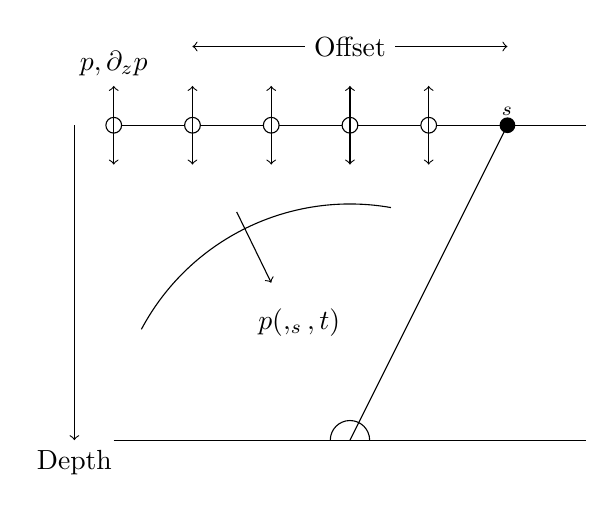
\begin{tikzpicture}[scale=1.0]
  \draw[->] (-0.5,4.0) -- (-0.5,0.0) node[below]{Depth} ;     %Draw Depth axis
  \draw[<->] (1.0,5.0) -- node[fill=white]{Offset} (5.0,5.0); %Draw offset axis 
  \draw (0.0,0.0) -- (6.0,0.0) ;  %Top boundary
  \draw (0.0,4.0) -- (6.0,4.0) ;  %Bottom boundary

  \fill (5.0,4.0) node[above]{$\xx_s$} circle (0.1) ; % Draw source

  \fill[white] (0.0,4.0) circle (0.1) ; %Draw receiver
  \draw (0.0,4.0) circle (0.1) ;
  \draw[->] (0.0,4.0) -- (0.0,4.5);
  \draw[->] (0.0,4.0) -- (0.0,3.5);
  \draw (0.0,4.5) node[above]{$p,\partial_z p$};
  

  \fill[white](1.0,4.0) circle (0.1) ;
  \draw (1.0,4.0) node[above]{} circle (0.1) ;
  \draw[->] (1.0,4.0) -- (1.0,4.5);
  \draw[->] (1.0,4.0) -- (1.0,3.5);

  \fill[white] (2.0,4.0) circle (0.1) ;
  \draw (2.0,4.0) circle (0.1) ;
  \draw[->] (2.0,4.0) -- (2.0,4.5);
  \draw[->] (2.0,4.0) -- (2.0,3.5);

  \fill[white] (3.0,4.0) circle (0.1) ;
  \draw (3.0,4.0) circle (0.1) ;
  \draw[->] (3.0,4.0) -- (3.0,4.5);
  \draw[->] (3.0,4.0) -- (3.0,3.5);

  \fill[white] (4.0,4.0) circle (0.1) ;
  \draw (4.0,4.0) circle (0.1) ;
  \draw[->] (4.0,4.0) -- (4.0,4.5);
  \draw[->] (4.0,4.0) -- (4.0,3.5);

  \draw[<-] (2,2)-- +(116:1);
  \draw (3,0) +(0:0.25) arc(0:180:0.25);
  \draw (3,0) +(80:3) arc(80:152:3);
  \draw (3.0,1.5) node[left]{$p(\xx,\xx_s,t)$};


  \draw (5.0,4.0) -- (3.0,0.0) ;
  %\draw (3.0,0.0) -- (1.0,4.0) ;
\end{tikzpicture}
%\label{fig:si-1}

$p$: Scattered wavefield \\
$\xx_s$: Source position\\
$\xx,t$: Position,time
\end{figure}
\end{frame}
%-----------------------------------------
\begin{frame}{Imaging condition IV}
%-----------------------------------------
\begin{figure}
\begin{tikzpicture}[scale=1.0]
  \draw[->] (-0.5,4.0) -- (-0.5,0.0) node[below]{Depth} ;     %Draw Depth axis
  \draw[<->] (1.0,5.0) -- node[fill=white]{Offset} (5.0,5.0); %Draw offset axis 
  \draw (0.0,0.0) -- (6.0,0.0) ;  %Top boundary
  \draw (0.0,4.0) -- (6.0,4.0) ;  %Bottom boundary

  \fill (5.0,4.0) node[above]{$\xx_s$} circle (0.1) ; % Draw source

  \fill[white] (0.0,0.5) circle (0.1) ; %Draw receiver
  \draw (0.0,0.5) circle (0.1) ;
  

  \fill[white](1.0,0.5) circle (0.1) ;
  \draw (1.0,0.5) node[above]{} circle (0.1) ;

  \fill[white] (2.0,0.5) circle (0.1) ;
  \draw (2.0,0.5) circle (0.1) ;

%  \fill[white] (3.0,0.5) circle (0.1) ;
%  \draw (3.0,0.5) circle (0.1) ;

%  \fill[white] (4.0,0.5) circle (0.1) ;
%  \draw (4.0,0.5) circle (0.1) ;

  \draw[->] (3,0)-- (0.0,0.5);
  \draw[->] (3,0)-- (1.0,0.5);
  \draw[->] (3,0)-- (2.0,0.5);
  %\draw[->] (3,0)-- (3.0,0.5);
  %\draw[->] (3,0)-- (4.0,0.5);
%  \draw (3,0) +(0:0.25) arc(0:180:0.25);
%  \draw (3,0) +(80:3) arc(80:152:3);
  \draw (3.0,1.5) node[left]{$p(\xx,\xx_s,t)$};


  \draw (5.0,4.0) -- (3.0,0.0) ;
  %\draw (3.0,0.0) -- (1.0,4.0) ;
\end{tikzpicture}
%\label{fig:si-1}
\end{figure}
\end{frame}
%-----------------------------------------
\begin{frame}{Imaging condition V}
%-----------------------------------------
\begin{figure}
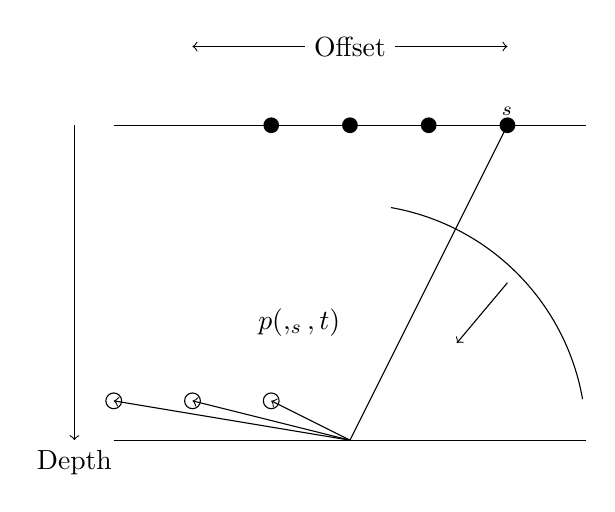
\begin{tikzpicture}[scale=1.0]
  \draw[->] (-0.5,4.0) -- (-0.5,0.0) node[below]{Depth} ;     %Draw Depth axis
  \draw[<->] (1.0,5.0) -- node[fill=white]{Offset} (5.0,5.0); %Draw offset axis 
  \draw (0.0,0.0) -- (6.0,0.0) ;  %Top boundary
  \draw (0.0,4.0) -- (6.0,4.0) ;  %Bottom boundary

  \fill (5.0,4.0) node[above]{$\xx_s$} circle (0.1) ; % Draw source
  \fill (4.0,4.0) node[above]{} circle (0.1) ; % Draw source
  \fill (3.0,4.0) node[above]{} circle (0.1) ; % Draw source
  \fill (2.0,4.0) node[above]{} circle (0.1) ; % Draw source

  \fill[white] (0.0,0.5) circle (0.1) ; %Draw receiver
  \draw (0.0,0.5) circle (0.1) ;
  

  \fill[white](1.0,0.5) circle (0.1) ;
  \draw (1.0,0.5) node[above]{} circle (0.1) ;

  \fill[white] (2.0,0.5) circle (0.1) ;
  \draw (2.0,0.5) circle (0.1) ;

%  \fill[white] (3.0,0.5) circle (0.1) ;
%  \draw (3.0,0.5) circle (0.1) ;

%  \fill[white] (4.0,0.5) circle (0.1) ;
%  \draw (4.0,0.5) circle (0.1) ;

  \draw[->] (3,0)-- (0.0,0.5);
  \draw[->] (3,0)-- (1.0,0.5);
  \draw[->] (3,0)-- (2.0,0.5);
%  \draw[->] (3,0)-- (3.0,0.5);
%  \draw[->] (3,0)-- (4.0,0.5);
%  \draw (3,0) +(0:0.25) arc(0:180:0.25);
%  \draw (3,0) +(80:3) arc(80:152:3);
  \draw (3.0,1.5) node[left]{$p(\xx,\xx_s,t)$};
\draw (3,0) +(80:3) arc(80:10:3);

  \draw[->] (5,2)-- +(230:1);

  \draw (5.0,4.0) -- (3.0,0.0) ;
  %\draw (3.0,0.0) -- (1.0,4.0) ;
\end{tikzpicture}
%\label{fig:si-1}
\end{figure}
\end{frame}
%-----------------------------------------
\begin{frame}{Imaging condition VI}
%-----------------------------------------
\begin{figure}
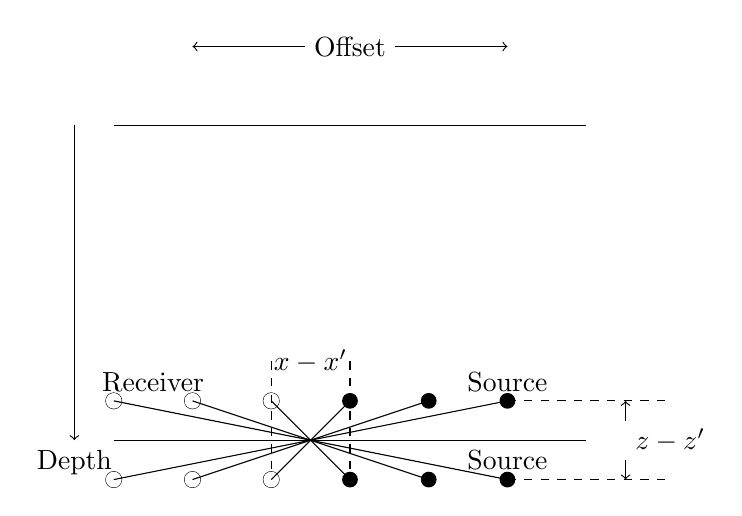
\begin{tikzpicture}[scale=1.0]
   \draw[->] (-0.5,4.0) -- (-0.5,0.0) node[below]{Depth} ;      %Depth axis 
   \draw[<->] (1.0,5.0) -- node[fill=white]{Offset} (5.0,5.0);  %Offset axis  
  \draw (0.0,4.0) -- (6.0,4.0) ;                               % Boundary at top
  \draw (0.0,0.0) -- (6.0,0.0) ;                               % Boundary at depth

  \fill (3.0,0.5) node[above]{} circle (0.1) ;           % Draw source
  \fill (4.0,0.5) node[above]{} circle (0.1) ;           % Draw source
  \fill (5.0,0.5) node[above]{Source} circle (0.1) ;     % Draw source text

  \draw (2.0,0.5) circle (0.1) ;             %Draw receiver
  \fill[white] (2.0,0.5) circle (0.1) ;

  \draw (1.0,0.5) circle (0.1) ;             %Draw receiver
  \fill[white] (1.0,0.5) circle (0.1) ;

  \draw (0.0,0.5) circle (0.1) ;             %Draw receiver
  \fill[white] (0.0,0.5) circle (0.1) ;
  \draw (0.5,0.5) node[above]{Receiver} ;    %Draw receiver text 

  \draw (3.0,0.5) -- (2.5,0.0);              % Draw ray from source to midpoint
  \draw (4.0,0.5) -- (2.5,0.0);              % Draw ray from source to midpoint
  \draw (5.0,0.5) -- (2.5,0.0);              % Draw ray from source to midpoint

  \draw (2.0,0.5) -- (2.5,0.0);              % Draw ray from receiver to midpoint
  \draw (1.0,0.5) -- (2.5,0.0);              % Draw ray from receiver to midpoint
  \draw (0.0,0.5) -- (2.5,0.0);              % Draw ray from receiver to midpoint

  \draw[dashed] (2.0,1.0) -- (2.0,-0.5);     %Draw vertical dashed line
  \draw[dashed] (3.0,1.0) -- (3.0,-0.5);     %Draw vertical dashed line
  \draw (2.5,1.0) node {$x-x'$};           % Draw equation
  \draw[dashed] (5.0,0.5) -- (7.0,0.5);     %Draw vertical dashed line
  \draw[dashed] (5.0,-0.5) -- (7.0,-0.5);     %Draw vertical dashed line
  \draw (6.5,0.0) node[right]{$z-z'$};           % Draw equation
  \draw[->] (6.5,0.25) -- (6.5,0.5);
  \draw[->] (6.5,-0.25) -- (6.5,-0.5);



  \fill (3.0,-0.5) node[above]{} circle (0.1) ;           % Draw source
  \fill (4.0,-0.5) node[above]{} circle (0.1) ;           % Draw source
  \fill (5.0,-0.5) node[above]{Source} circle (0.1) ;     % Draw source text

  \draw (2.0,-0.5) circle (0.1) ;             %Draw receiver
  \fill[white] (2.0,-0.5) circle (0.1) ;

  \draw (1.0,-0.5) circle (0.1) ;             %Draw receiver
  \fill[white] (1.0,-0.5) circle (0.1) ;

  \draw (0.0,-0.5) circle (0.1) ;             %Draw receiver
  \fill[white] (0.0,-0.5) circle (0.1) ;
  %\draw (0.5,0.5) node[above]{Receiver} ;    %Draw receiver text 

  \draw (3.0,-0.5) -- (2.5,0.0);              % Draw ray from source to midpoint
  \draw (4.0,-0.5) -- (2.5,0.0);              % Draw ray from source to midpoint
  \draw (5.0,-0.5) -- (2.5,0.0);              % Draw ray from source to midpoint

  \draw (2.0,-0.5) -- (2.5,0.0);              % Draw ray from receiver to midpoint
  \draw (1.0,-0.5) -- (2.5,0.0);              % Draw ray from receiver to midpoint
  \draw (0.0,-0.5) -- (2.5,0.0);              % Draw ray from receiver to midpoint
\end{tikzpicture}
\end{figure}

$x-x'$: Horizontal offset \\
$z-z'$: Vertical offset 
\end{frame}
%-----------------------------------------
\begin{frame}{Numerical example}
%-----------------------------------------
Reflectivity $p(\xx-\xx',t=0)$ at all depths
using new imaging condition
%
\begin{figure}
\epsfig{file=Fig/cip-1-ta,width=8cm}
\end{figure}
\end{frame}
%-----------------------------------------
\begin{frame}{Numerical example}
%-----------------------------------------
Full section $p(\xx-\xx'=0,t)$ at all depths
using new imaging condition
%
\begin{figure}
\epsfig{file=Fig/sect-ta,width=8cm}
\end{figure}
\end{frame}
%---------------------------------
\begin{frame}{Simplification}
%---------------------------------
\begin{eqnarray}
 r(\xx',\xx,t=0)=\nonumber\\
\int dS(\xx_s)\, \int d\tau\, \left[p(\xx',\xx_s,\tau)\nabla p_0(\xx,\xx_s,\tau)\right.\nonumber\\
   -\left. p_0(\xx,\xx_s,\tau)\nabla p(\xx',\xx_s,\tau)\right]\cdot \nn(\xx')
&&                   \label{eq:10400}
\end{eqnarray}
Horizontal receiver implies 
\begin{eqnarray}
 r(\xx',\xx,t=0)=\nonumber\\
\int dS(\xx_s)\, \int d\tau\, \left[p(\xx',\xx_s,\tau)\partial_z p_0(\xx,\xx_s,\tau)\right.\nonumber\\
   -\left. p_0(\xx,\xx_s,\tau)\partial_z' p(\xx',\xx_s,\tau)\right]
&&                   \label{eq:10500}
\end{eqnarray}
\end{frame}
%---------------------------------
\begin{frame}{Simplification}
%---------------------------------
$\partial_z p(\xx',\xx_s.t)=0$ (No recorded pressure gradient)
\begin{eqnarray}
 r(\xx',\xx,t=0)=\nonumber\\
\int dS(\xx_s)\, \int d\tau\, \left[p(\xx',\xx_s,\tau)\partial_z p_0(\xx,\xx_s,\tau)\right.\nonumber\\
&&                   \label{eq:10600}
\end{eqnarray}
\end{frame}
%-----------------------------------------
\begin{frame}{Classical Imaging condition}
%-----------------------------------------
For $\xx'=\xx$ and by ignoring $\partial_z$ this is the classical imaging condition (Claerbout, 1971)
\begin{eqnarray}
  r_{c}(\xx) =
    \sum_{\xx_s}\sum_{\tau}p_0(\xx,\xx_s,\tau)p(\xx,\xx_s,\tau)\nonumber\\ 
                                                 \nonumber
\end{eqnarray}
Ignoring $\partial_z$ implies an unfocused image with 
less than optimal resolution and incorrect amplitudes.
\end{frame}
%------------------------------------------------------
\begin{frame}{Numerical examples}
%------------------------------------------------------
Common image point gather (CIP) in the center of the model
Classical imaging condition: 
\begin{figure}
\epsfig{file=Fig/case-1-cig,width=9cm}
\end{figure}
\end{frame}
%------------------------------------------------------
\begin{frame}{Numerical examples}
%------------------------------------------------------
Horizontal profile through reflector at 1000m depth
\begin{figure}
\epsfig{file=Fig/case-1-cig-h,width=9cm}
\end{figure}
\end{frame}
%------------------------------------------------------
\begin{frame}{Numerical examples}
%------------------------------------------------------
Common image point gather (CIP) in the center of the model.\\
New imaging condition: 
\begin{figure}
\epsfig{file=Fig/case-2-cig,width=9cm}
\end{figure}
\end{frame}
%------------------------------------------------------
\begin{frame}{Numerical examples}
%------------------------------------------------------
Horizontal profile through reflector at 1000m depth
\begin{figure}
\epsfig{file=Fig/case-2-cig-h,width=9cm}
\end{figure}
\end{frame}
%------------------------------------------------------
\begin{frame}{Numerical example}
%------------------------------------------------------
Conventional imaging condition:
\begin{figure}
\epsfig{file=Fig/case-4-stack,width=10cm}
\end{figure}
\end{frame}
%------------------------------------------------------
\begin{frame}{Numerical example}
%------------------------------------------------------
New imaging condition:
\begin{figure}
\epsfig{file=Fig/case-5-stack,width=10cm}
\end{figure}
\end{frame}
%------------------------------------------------------
\begin{frame}{Numerical example}
%------------------------------------------------------
Conventional imaging condition:
\begin{figure}
\epsfig{file=Fig/case-4-stack-zoom,width=9cm}
\end{figure}
\end{frame}
%------------------------------------------------------
\begin{frame}{Numerical example}
%------------------------------------------------------
New imaging condition:
\begin{figure}
\epsfig{file=Fig/case-5-stack-zoom,width=9cm}
\end{figure}
\end{frame}
%------------------------------------------------------
\begin{frame}{Numerical example}
%------------------------------------------------------
From reflectivity to plane wave reflection coefficient
\begin{eqnarray}
  \partial_z r(\xx,\xx',t) & = & 
   2\sum_{\xx_s}\sum_{\tau}\d^2_{z_s} p_0(\xx,\xx_s,\tau+t)p_{sc}(\xx',\xx_s,\tau)
\end{eqnarray}
Plane wave reflection coefficient by mapping to $p-\tau$ (deBruin 1991\cite{Bruin1990}) 

\vspace{1cm}
Conventional approach:
\begin{eqnarray}
  r(\xx,\xx',t) & = & 
   2\sum_{\xx_s}\sum_{\tau}p_0(\xx,\xx_s,\tau+t)p_{sc}(\xx',\xx_s,\tau)
\end{eqnarray}
Plane wave reflection coefficient by mapping to $p-\tau$ (deBruin 1991\cite{Bruin1990}) 

\end{frame}
%------------------------------------------------------
\begin{frame}{Numerical example}
%------------------------------------------------------
$p$-gather at the center of the model
\begin{figure}
\epsfig{file=Fig/case-3-cag,width=10cm}
\end{figure}
\end{frame}
%------------------------------------------------------
\begin{frame}{Numerical example}
%------------------------------------------------------
Amplitude picks along $p$-gather
\begin{figure}
\epsfig{file=Fig/case-3-pick,width=10cm}
\end{figure}
\end{frame}
%------------------------------------------------------
\begin{frame}{Numerical example}
%------------------------------------------------------
Conventional approach:
\begin{figure}
\epsfig{file=Fig/case-1-cag,width=10cm}
\end{figure}
\end{frame}
%------------------------------------------------------
\begin{frame}{Numerical example}
%------------------------------------------------------
Amplitude picks along $p$-gather
\begin{figure}
\epsfig{file=Fig/case-1-pick,width=10cm}
\end{figure}
\end{frame}
%-----------------------------------------
\begin{frame}{Conclusions}
%-----------------------------------------
Simple (trivial) modification of the classical
imaging condition for Reverse-time migration gives
\begin{itemize}
  \item Better resolution
  \item Reflectivity with correct angle behavior
\end{itemize}
\end{frame}
\end{document}
